%*******************************************
% Lab 03: Priority Encoder
%*******************************************
\chapter{Priority Encoder}

\section{Purpose}

Often a circuit will receive data from several sources at one time and there must be a way to prioritize those inputs. This circuit creates a simple priority encoder for nine different inputs. This is a fairly simple circuit but is best explained by building and ``playing around'' with it rather than attempting to understand a printed text; thus, the explanation for this lab is somewhat limited.

\section{Procedure}

Start \textit{Logisim-evolution} and create a subcircuit named \lstinline[columns=fixed]|Encoder|. Open that subcircuit and place 12 \texttt{AND} gates as illustrated in Figure \ref{fig:03-01}.

\begin{figure}[H]
	\centering
	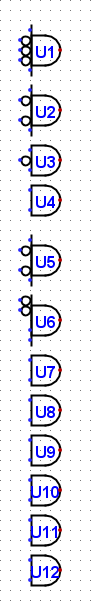
\includegraphics[width=\maxwidth{.95\linewidth}]{gfx/03-01}
	\caption{AND Gates}
	\label{fig:03-01}
\end{figure}

The gates have one data bit and these properties:

\begin{itemize}
	\item \textbf{U1}: Five inputs, numbers two, three, and four negated.
	\item \textbf{U2}: Four inputs, numbers two and three negated.
	\item \textbf{U3}: Three inputs, number two negated.
	\item \textbf{U4}: Two inputs, none negated.
	\item \textbf{U5}: Four inputs, numbers two and three negated.
	\item \textbf{U6}: Four inputs, numbers one and two negated.
	\item \textbf{U7-U12}: Two inputs, none negated. 
\end{itemize}

Many of the output signals need to be combined with \texttt{OR} gates and those should be added next, as in Figure \ref{fig:03-02}. Note: U16 is a \texttt{NOR} (\textit{Gates} library) gate.

\begin{figure}[H]
	\centering
	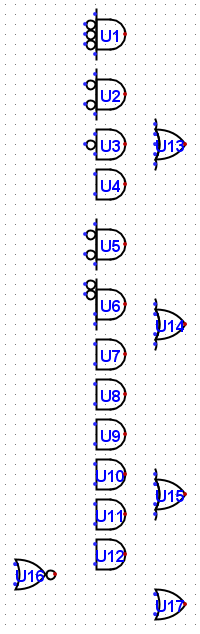
\includegraphics[width=\maxwidth{.95\linewidth}]{gfx/03-02}
	\caption{OR Gates Added}
	\label{fig:03-02}
\end{figure}

This encoder is designed to prioritize nine input lines so nine inputs must be added, as illustrated in Figure 

\begin{figure}[H]
	\centering
	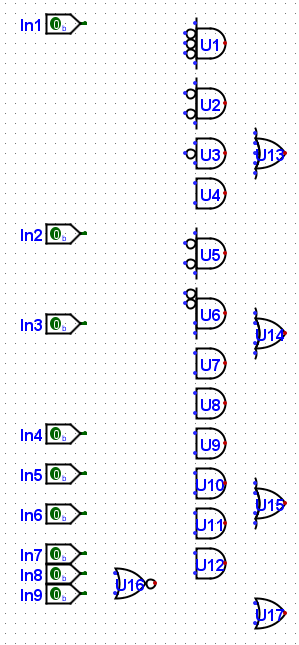
\includegraphics[width=\maxwidth{.95\linewidth}]{gfx/03-03}
	\caption{Inputs Added}
	\label{fig:03-03}
\end{figure}

Wiring this circuit is the most challenging part of the build. As illustrated in Figure \ref{fig:03-04}, the inputs are wired to several different \texttt{AND} gates.

\begin{figure}[H]
	\centering
	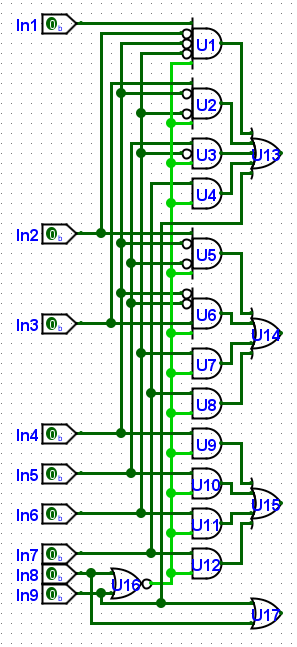
\includegraphics[width=\maxwidth{.95\linewidth}]{gfx/03-04}
	\caption{Wiring the Encoder}
	\label{fig:03-04}
\end{figure}

Finally, four output ports are added, as illustrated in Figure \ref{fig:03-05}. 

\begin{figure}[H]
	\centering
	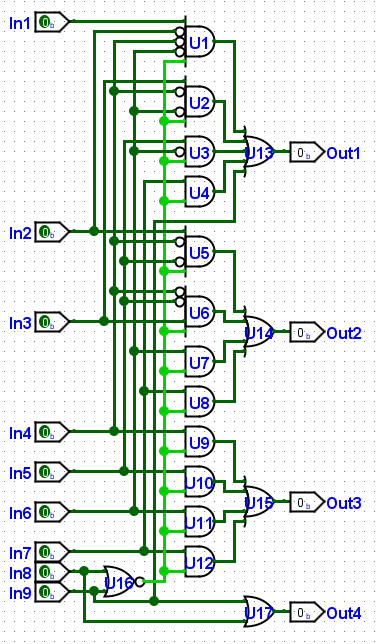
\includegraphics[width=\maxwidth{.95\linewidth}]{gfx/03-05}
	\caption{Nine-line Priority Encoder}
	\label{fig:03-05}
\end{figure}

This circuit is designed to output a \acf{BCD} number, so no further conversion is needed to be able to read the highest priority input line. At this point, the circuit is complete and the \textit{poke} tool can be used to change the inputs and observe how that high input bit drives the outputs.

To finish the project, open the \lstinline[columns=fixed]|main| circuit and drop the \lstinline[columns=fixed]|Encoder| on the drawing canvas. Add nine inputs and label them \textit{In1} through \textit{In9}. Place a Hex Digit Display (\textit{Input/Output} library) and wire the four outputs through a splitter to that display. The \lstinline[columns=fixed]|main| circuit is illustrated in Figure \ref{fig:03-06}.

\begin{figure}[H]
	\centering
	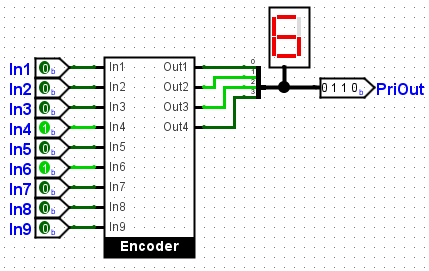
\includegraphics[width=\maxwidth{.95\linewidth}]{gfx/03-06}
	\caption{Main Circuit}
	\label{fig:03-06}
\end{figure}


\subsection{Testing the Circuit}

The circuit is now complete. It should be tested by entering various combinations of inputs and observing that the output always displays the highest numbered input. For example, in Figure \ref{fig:03-06} the output displays ``6'' even though both \textit{In4} and \textit{In6} are high.

\section{Deliverable}

To receive a grade for this lab, create the Nine-line Priority Encoder circuit as defined in this lab. Be sure the standard identifying information is at the top left of the circuit, similar to this:

\bigskip
% The minipage environment keeps the three lines together - no page break.
\begin{minipage}{\linewidth}
	\begin{verbatim}
	George Self
	Lab 03: Nine-line Priority Encoder
	February 18, 2018
	\end{verbatim}
\end{minipage}
\bigskip

Save the file with this name: \emph{\texttt{Lab03\_Encoder}} and submit that file for grading.